\documentclass[onecolumn, draftclsnofoot,10pt, compsoc]{IEEEtran}
\usepackage{graphicx}
\usepackage{url}
\usepackage{setspace}
\usepackage{enumitem}
\usepackage{geometry}
\usepackage{pgfgantt}
% \usepackage{tabularx}
\usepackage{longtable}

% \usepackage{float}
\usepackage{caption}
\usepackage{subfig}
\usepackage{listings}
\usepackage{changepage}
\usepackage{floatrow}
\usepackage{minted}
\floatsetup[listing]{style=Plaintop, font=bf}    

\captionsetup{justification=centering,font=bf}

\usepackage{fancyvrb}
\usepackage{color}
\usepackage[latin1]{inputenc}


\makeatletter
\def\PY@reset{\let\PY@it=\relax \let\PY@bf=\relax%
    \let\PY@ul=\relax \let\PY@tc=\relax%
    \let\PY@bc=\relax \let\PY@ff=\relax}
\def\PY@tok#1{\csname PY@tok@#1\endcsname}
\def\PY@toks#1+{\ifx\relax#1\empty\else%
    \PY@tok{#1}\expandafter\PY@toks\fi}
\def\PY@do#1{\PY@bc{\PY@tc{\PY@ul{%
    \PY@it{\PY@bf{\PY@ff{#1}}}}}}}
\def\PY#1#2{\PY@reset\PY@toks#1+\relax+\PY@do{#2}}

\expandafter\def\csname PY@tok@gd\endcsname{\def\PY@tc##1{\textcolor[rgb]{0.63,0.00,0.00}{##1}}}
\expandafter\def\csname PY@tok@gu\endcsname{\let\PY@bf=\textbf\def\PY@tc##1{\textcolor[rgb]{0.50,0.00,0.50}{##1}}}
\expandafter\def\csname PY@tok@gt\endcsname{\def\PY@tc##1{\textcolor[rgb]{0.00,0.25,0.82}{##1}}}
\expandafter\def\csname PY@tok@gs\endcsname{\let\PY@bf=\textbf}
\expandafter\def\csname PY@tok@gr\endcsname{\def\PY@tc##1{\textcolor[rgb]{1.00,0.00,0.00}{##1}}}
\expandafter\def\csname PY@tok@cm\endcsname{\let\PY@it=\textit\def\PY@tc##1{\textcolor[rgb]{0.25,0.50,0.50}{##1}}}
\expandafter\def\csname PY@tok@vg\endcsname{\def\PY@tc##1{\textcolor[rgb]{0.10,0.09,0.49}{##1}}}
\expandafter\def\csname PY@tok@m\endcsname{\def\PY@tc##1{\textcolor[rgb]{0.40,0.40,0.40}{##1}}}
\expandafter\def\csname PY@tok@mh\endcsname{\def\PY@tc##1{\textcolor[rgb]{0.40,0.40,0.40}{##1}}}
\expandafter\def\csname PY@tok@go\endcsname{\def\PY@tc##1{\textcolor[rgb]{0.50,0.50,0.50}{##1}}}
\expandafter\def\csname PY@tok@ge\endcsname{\let\PY@it=\textit}
\expandafter\def\csname PY@tok@vc\endcsname{\def\PY@tc##1{\textcolor[rgb]{0.10,0.09,0.49}{##1}}}
\expandafter\def\csname PY@tok@il\endcsname{\def\PY@tc##1{\textcolor[rgb]{0.40,0.40,0.40}{##1}}}
\expandafter\def\csname PY@tok@cs\endcsname{\let\PY@it=\textit\def\PY@tc##1{\textcolor[rgb]{0.25,0.50,0.50}{##1}}}
\expandafter\def\csname PY@tok@cp\endcsname{\def\PY@tc##1{\textcolor[rgb]{0.74,0.48,0.00}{##1}}}
\expandafter\def\csname PY@tok@gi\endcsname{\def\PY@tc##1{\textcolor[rgb]{0.00,0.63,0.00}{##1}}}
\expandafter\def\csname PY@tok@gh\endcsname{\let\PY@bf=\textbf\def\PY@tc##1{\textcolor[rgb]{0.00,0.00,0.50}{##1}}}
\expandafter\def\csname PY@tok@ni\endcsname{\let\PY@bf=\textbf\def\PY@tc##1{\textcolor[rgb]{0.60,0.60,0.60}{##1}}}
\expandafter\def\csname PY@tok@nl\endcsname{\def\PY@tc##1{\textcolor[rgb]{0.63,0.63,0.00}{##1}}}
\expandafter\def\csname PY@tok@nn\endcsname{\let\PY@bf=\textbf\def\PY@tc##1{\textcolor[rgb]{0.00,0.00,1.00}{##1}}}
\expandafter\def\csname PY@tok@no\endcsname{\def\PY@tc##1{\textcolor[rgb]{0.53,0.00,0.00}{##1}}}
\expandafter\def\csname PY@tok@na\endcsname{\def\PY@tc##1{\textcolor[rgb]{0.49,0.56,0.16}{##1}}}
\expandafter\def\csname PY@tok@nb\endcsname{\def\PY@tc##1{\textcolor[rgb]{0.00,0.50,0.00}{##1}}}
\expandafter\def\csname PY@tok@nc\endcsname{\let\PY@bf=\textbf\def\PY@tc##1{\textcolor[rgb]{0.00,0.00,1.00}{##1}}}
\expandafter\def\csname PY@tok@nd\endcsname{\def\PY@tc##1{\textcolor[rgb]{0.67,0.13,1.00}{##1}}}
\expandafter\def\csname PY@tok@ne\endcsname{\let\PY@bf=\textbf\def\PY@tc##1{\textcolor[rgb]{0.82,0.25,0.23}{##1}}}
\expandafter\def\csname PY@tok@nf\endcsname{\def\PY@tc##1{\textcolor[rgb]{0.00,0.00,1.00}{##1}}}
\expandafter\def\csname PY@tok@si\endcsname{\let\PY@bf=\textbf\def\PY@tc##1{\textcolor[rgb]{0.73,0.40,0.53}{##1}}}
\expandafter\def\csname PY@tok@s2\endcsname{\def\PY@tc##1{\textcolor[rgb]{0.73,0.13,0.13}{##1}}}
\expandafter\def\csname PY@tok@vi\endcsname{\def\PY@tc##1{\textcolor[rgb]{0.10,0.09,0.49}{##1}}}
\expandafter\def\csname PY@tok@nt\endcsname{\let\PY@bf=\textbf\def\PY@tc##1{\textcolor[rgb]{0.00,0.50,0.00}{##1}}}
\expandafter\def\csname PY@tok@nv\endcsname{\def\PY@tc##1{\textcolor[rgb]{0.10,0.09,0.49}{##1}}}
\expandafter\def\csname PY@tok@s1\endcsname{\def\PY@tc##1{\textcolor[rgb]{0.73,0.13,0.13}{##1}}}
\expandafter\def\csname PY@tok@sh\endcsname{\def\PY@tc##1{\textcolor[rgb]{0.73,0.13,0.13}{##1}}}
\expandafter\def\csname PY@tok@sc\endcsname{\def\PY@tc##1{\textcolor[rgb]{0.73,0.13,0.13}{##1}}}
\expandafter\def\csname PY@tok@sx\endcsname{\def\PY@tc##1{\textcolor[rgb]{0.00,0.50,0.00}{##1}}}
\expandafter\def\csname PY@tok@bp\endcsname{\def\PY@tc##1{\textcolor[rgb]{0.00,0.50,0.00}{##1}}}
\expandafter\def\csname PY@tok@c1\endcsname{\let\PY@it=\textit\def\PY@tc##1{\textcolor[rgb]{0.25,0.50,0.50}{##1}}}
\expandafter\def\csname PY@tok@kc\endcsname{\let\PY@bf=\textbf\def\PY@tc##1{\textcolor[rgb]{0.00,0.50,0.00}{##1}}}
\expandafter\def\csname PY@tok@c\endcsname{\let\PY@it=\textit\def\PY@tc##1{\textcolor[rgb]{0.25,0.50,0.50}{##1}}}
\expandafter\def\csname PY@tok@mf\endcsname{\def\PY@tc##1{\textcolor[rgb]{0.40,0.40,0.40}{##1}}}
\expandafter\def\csname PY@tok@err\endcsname{\def\PY@bc##1{\setlength{\fboxsep}{0pt}\fcolorbox[rgb]{1.00,0.00,0.00}{1,1,1}{\strut ##1}}}
\expandafter\def\csname PY@tok@kd\endcsname{\let\PY@bf=\textbf\def\PY@tc##1{\textcolor[rgb]{0.00,0.50,0.00}{##1}}}
\expandafter\def\csname PY@tok@ss\endcsname{\def\PY@tc##1{\textcolor[rgb]{0.10,0.09,0.49}{##1}}}
\expandafter\def\csname PY@tok@sr\endcsname{\def\PY@tc##1{\textcolor[rgb]{0.73,0.40,0.53}{##1}}}
\expandafter\def\csname PY@tok@mo\endcsname{\def\PY@tc##1{\textcolor[rgb]{0.40,0.40,0.40}{##1}}}
\expandafter\def\csname PY@tok@kn\endcsname{\let\PY@bf=\textbf\def\PY@tc##1{\textcolor[rgb]{0.00,0.50,0.00}{##1}}}
\expandafter\def\csname PY@tok@mi\endcsname{\def\PY@tc##1{\textcolor[rgb]{0.40,0.40,0.40}{##1}}}
\expandafter\def\csname PY@tok@gp\endcsname{\let\PY@bf=\textbf\def\PY@tc##1{\textcolor[rgb]{0.00,0.00,0.50}{##1}}}
\expandafter\def\csname PY@tok@o\endcsname{\def\PY@tc##1{\textcolor[rgb]{0.40,0.40,0.40}{##1}}}
\expandafter\def\csname PY@tok@kr\endcsname{\let\PY@bf=\textbf\def\PY@tc##1{\textcolor[rgb]{0.00,0.50,0.00}{##1}}}
\expandafter\def\csname PY@tok@s\endcsname{\def\PY@tc##1{\textcolor[rgb]{0.73,0.13,0.13}{##1}}}
\expandafter\def\csname PY@tok@kp\endcsname{\def\PY@tc##1{\textcolor[rgb]{0.00,0.50,0.00}{##1}}}
\expandafter\def\csname PY@tok@w\endcsname{\def\PY@tc##1{\textcolor[rgb]{0.73,0.73,0.73}{##1}}}
\expandafter\def\csname PY@tok@kt\endcsname{\def\PY@tc##1{\textcolor[rgb]{0.69,0.00,0.25}{##1}}}
\expandafter\def\csname PY@tok@ow\endcsname{\let\PY@bf=\textbf\def\PY@tc##1{\textcolor[rgb]{0.67,0.13,1.00}{##1}}}
\expandafter\def\csname PY@tok@sb\endcsname{\def\PY@tc##1{\textcolor[rgb]{0.73,0.13,0.13}{##1}}}
\expandafter\def\csname PY@tok@k\endcsname{\let\PY@bf=\textbf\def\PY@tc##1{\textcolor[rgb]{0.00,0.50,0.00}{##1}}}
\expandafter\def\csname PY@tok@se\endcsname{\let\PY@bf=\textbf\def\PY@tc##1{\textcolor[rgb]{0.73,0.40,0.13}{##1}}}
\expandafter\def\csname PY@tok@sd\endcsname{\let\PY@it=\textit\def\PY@tc##1{\textcolor[rgb]{0.73,0.13,0.13}{##1}}}

\def\PYZbs{\char`\\}
\def\PYZus{\char`\_}
\def\PYZob{\char`\{}
\def\PYZcb{\char`\}}
\def\PYZca{\char`\^}
\def\PYZam{\char`\&}
\def\PYZlt{\char`\<}
\def\PYZgt{\char`\>}
\def\PYZsh{\char`\#}
\def\PYZpc{\char`\%}
\def\PYZdl{\char`\$}
\def\PYZti{\char`\~}
% for compatibility with earlier versions
\def\PYZat{@}
\def\PYZlb{[}
\def\PYZrb{]}
\makeatother



\geometry{textheight=9.5in, textwidth=7in}

\usepackage[parfill]{parskip}


% \newcommand{\subparagraph}{}

% % Reformat section and subsection styles
% \usepackage{titlesec}
% \setcounter{secnumdepth}{4}

% \titleformat{\section}
% {\normalfont\huge\bfseries\sffamily}{\thesection}{1em}{}

% \titleformat{\subsection}
% {\normalfont\large\bfseries\sffamily}{\thesubsection}{1em}{}

% \titleformat{\subsubsection}
% {\normalfont\normalsize\bfseries\sffamily}{\thesubsubsection}{1em}{}

% \titleformat{\paragraph}
% {\normalfont\normalsize\sffamily\itshape}{\theparagraph}{2em}{}


% 1. Fill in these details
\def \CapstoneTeamName{     }
\def \CapstoneTeamNumber{       36}
\def \GroupMemberOne{           Trevor Swope}
\def \GroupMemberTwo{           William Selbie}
\def \GroupMemberThree{         Luke Goertzen}
\def \CapstoneProjectName{      Project LOOM}
\def \CapstoneSponsorCompany{   Openly Published Environmental Sensing Lab}
\def \CapstoneSponsorPerson{    Chet Udell}

% 2. Uncomment the appropriate line below so that the document type works
\def \DocType{  %Problem Statement
                %Requirements Document
                % Technology Review
                % Preliminary Design Document
                Progress Report
                }
            
\newcommand{\NameSigPair}[1]{\par
\makebox[2.75in][r]{#1} \hfil   \makebox[3.25in]{\makebox[2.25in]{\hrulefill} \hfill        \makebox[.75in]{\hrulefill}}
\par\vspace{-12pt} \textit{\tiny\noindent
\makebox[2.75in]{} \hfil        \makebox[3.25in]{\makebox[2.25in][r]{Signature} \hfill  \makebox[.75in][r]{Date}}}}
% 3. If the document is not to be signed, uncomment the RENEWcommand below
%\renewcommand{\NameSigPair}[1]{#1}

%%%%%%%%%%%%%%%%%%%%%%%%%%%%%%%%%%%%%%%
\begin{document}
\begin{titlepage}
    \pagenumbering{gobble}
    \begin{singlespace}
        % \includegraphics[height=4cm]{coe_v_spot1}
        \hfill 
        % 4. If you have a logo, use this includegraphics command to put it on the coversheet.
        %\includegraphics[height=4cm]{CompanyLogo}   
        \par\vspace{.2in}
        \centering
        \scshape{
            \huge CS Capstone \DocType \par
            {\large\today}\par
            \vspace{.5in}
            \textbf{\Huge\CapstoneProjectName}\par
            \vfill
            {\large Prepared for}\par
            \Huge Kevin McGrath \\ Kirsten Winters \par
            \vspace{5pt}
            % {\Large\NameSigPair{\CapstoneSponsorPerson}\par}
            {\large Prepared by }\par
            Group\CapstoneTeamNumber\par
            % 5. comment out the line below this one if you do not wish to name your team
            \CapstoneTeamName\par 
            \vspace{5pt}
            % {\Large
            %     \NameSigPair{\GroupMemberOne}\par
            %     \NameSigPair{\GroupMemberTwo}\par
            %     \NameSigPair{\GroupMemberThree}\par
            % }
            \GroupMemberOne \\
            \GroupMemberTwo \\
            \GroupMemberThree \\
            \vspace{20pt}
        }
        \begin{abstract}
            A progress report of Senior Capstone Group 36's work for the duration of the Fall term. The report reiterates the goals of Project LOOM, describes the current status of the project and enumerates how this state was reached, with any problems and solutions in the process.
        \end{abstract}     
    \end{singlespace}
\end{titlepage}
\newpage
\pagenumbering{arabic}
\tableofcontents
% 7. uncomment this (if applicable). Consider adding a page break.
\listoffigures
\listoflistings
% \listoftables
\clearpage

\section{Project Purpose and Goals}
\subsection{Overview}  
    The Internet of Things (IoT) is a relatively new concept, entailing an aggregate of embedded systems capable of reading, transmitting, receiving, processing, or acting upon data. This often takes the form of a network of remotely connected devices that can be used for the purpose of autonomous data collection, or remote control and automation of various systems. One of the current restrictions that people and businesses face when seeking to develop IoT solutions is that, even for a simple project, there is a fairly high level of expertise required to implement it; this technical barrier becomes more and more prohibitive with systems of increasingly complex functionality.

    In other words, while anybody might have an idea for an Internet of Things project, not everybody has the technological knowledge and programming skills required to set it up, or the budget to contract it out to someone who does. The significance of this problem is that the technical barrier limits the pool of ideas and solutions that can be actualize through IoT. This means that problems that could have been solved are going unsolved because the people with the ideas to fix them do not have the means do so. With Project LOOM, we hope to create a system that is simple enough for anyone to use, but limitless in scale and complexity. In order to be perfectly scalable and infinite in scope, experienced users and virtuosos must have the ability to build their own modules and write their own code, otherwise, Project LOOM could not serve both beginners and experts.


\subsection{Goals}
    With Project LOOM, we aim to create an open-source, plug-and-play, suite of modular building blocks, the extensible and easy programmability of which expands the demographic of people capable of implementing Internet of Things solutions. For users with limited technical expertise to create complex systems, we aim to build a system that abstracts out the more technical details, allowing them to focus on their system more than the implementation of the modules. The system should also be usable by higher level students and experts by allowing them to modify or write their own firmware, and create new modules. Project LOOM will be developed for university faculty demos of functionality, possible subsequent commercialization is currently outside of the scope of the Senior Capstone project.

\section{Current Project Status}
    The project has progressed smoothly of the course of the last term, through strong organization and communication between the full Project LOOM group. So far, all of our client's goals for the term being met. 

    In terms of software, we have a functional user interface of data processors through MaxMSP, and know how to make more processors for new hardware or specialized needs as they arise. These processors can receive data from and send commands to Ishields on the network as OSC (Open Sound Control) bundles. Data processors have been developed to support attachments to Feather M0 WiFi, including: NeoPixel LED, servos, and MPU6050 boards with gyroscopes. We also have a simple processor to send calibration signals to Ishields.

    As far as firmware goes, we have enabled the FeatherM0 boards to act as WiFi access points on their own network, allowing the MaxMSP plugins to send packets to them. We have written routines for sending, receiving, and handling Open Sound Control bundles. We are able to send commands in the form of OSC bundles from Max to the actuators--right now, these are just the NeoPixel and the servos--and the actuators will work as expected. We are able to calibrate the MPU6050 with a command from MaxMSP and write those calibration values to flash memory so that the values are maintained if the device turns off. We are able to send data from the shields (mainly the MPU6050) to MaxMSP at regular intervals or on a request from the client, depending on what is selected in preprocessor statements on compile-time.

    Chet is planning on using using Project LOOM's current codebase and hardware for both his OSU Honors College class, and demos for faculty interested in IoT concepts, potentially to incorporate into their own courses.


    \begin{figure}[H]
        \centering
        \caption{Network Architecture}
        \label{fig:network_architecture}
        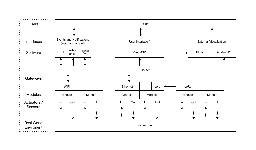
\includegraphics[width=16cm]{network_architecture.eps}         
    \end{figure}

\section{Weekly Summary}

\subsection{Week One}
\subsubsection*{Luke}
    \begin{adjustwidth}{2.5em}{0pt}
    \textbf{Summary -} This week was focused on setting up OneNote and reviewing and bidding upon proposals that we want to work on for the rest of the year. I turned in a copy of my resume for review. There is not much to report on currently.
    \end{adjustwidth}
\subsubsection*{Trevor}
    \begin{adjustwidth}{2.5em}{0pt}
    \textbf{Summary -} This week, I set up my OneNote unsuccessfully and then set it up successfully. I Approached Chet Udell with Will Selbie and Tyler Inberg and discussed the possibility of working on Project LOOM.
    \end{adjustwidth}
\subsubsection*{William}
    \begin{adjustwidth}{2.5em}{0pt}
    \textbf{Summary -} Approached Dr. Udell about working one Project LOOM. Set up OneNote.
    \end{adjustwidth}



\subsection{Week Two}
\subsubsection*{Luke}
    \begin{adjustwidth}{2.5em}{0pt}
    \textbf{Summary -} I received my project assignment (\#36 - Project Loom, client: Dr. Chet Udell), met with my team members but was unable to attend the first meeting with our client. Fortunately, it looks like we can meet again early next week so that I can produce a more comprehensive problem statement. Currently, logistics and organization seem to be going rather smoothly.
    
    \textbf{Problems -} I could not attend the full group meeting as I have class at that time.
    \end{adjustwidth}
    \begin{adjustwidth}{5em}{0pt}
    \textbf{Solution -} Got the meeting information from William and Trevor (and from reading the meeting notes taken by Thomas DeBell) and requested that an alternate time for meetings to be held.    
    \end{adjustwidth}
\subsubsection*{Trevor}
    \begin{adjustwidth}{2.5em}{0pt}
    \textbf{Summary -} Got assigned to Project LOOM with Group 36 (Luke Goertzen, Will Selbie) under Chet Udell. Met with Chet and he laid out the basic premise of the project, got added to BaseCamp for organizational things, divided the whole LOOM team into groups responsible for software, firmware, hardware, and the gateway layer of the project. I will be working primarily on firmware, but sometimes on software.
    \end{adjustwidth}
\subsubsection*{William}
    \begin{adjustwidth}{2.5em}{0pt}
    \textbf{Summary -} Scheduled weekly meetings on Tuesdays. Started using BaseCamp to keep track of assignments. Divided the LOOM team into smaller groups responsible for separate areas of the project (hardware, firmware, software, etc). Outlined the scope of the project.
    
    \textbf{Problems -} Finding a time for meetings that worked for everyone.
    \end{adjustwidth}
    \begin{adjustwidth}{5em}{0pt}
    \textbf{Solution -} Have multiple meetings each week to ensure everyone can make at least one meeting. 
    \end{adjustwidth}



\subsection{Week Three}
\subsubsection*{Luke}
    \begin{adjustwidth}{2.5em}{0pt}
    \textbf{Summary -} This week, we turned in our rough drafts of the problem statement which we will start combining to form our final draft next week. We had our first TA meeting and have scheduled a time for meetings with Chet, our client. We continued looking into tools we will be using for the project.
    
    \textbf{Problems -} Have not yet met with the our project's client, which is important for me to be able to finalize the problem statement.
    \end{adjustwidth}
    \begin{adjustwidth}{5em}{0pt}
    \textbf{Solution -} We scheduled Monday mornings for meetings of just the computer science team of Project LOOM.
    \end{adjustwidth}
\subsubsection*{Trevor}
    \begin{adjustwidth}{2.5em}{0pt}
    \textbf{Summary -} Turned in rough draft of problem statement. Met with TA Juneki Hong. Set up a time for meetings just with the CS Capstone team. Downloaded MaxMSP and started working through that a little bit. Met with Chet and he gave us a tour of some  of the prior work on the project (MaxMSP plugins, previous shields).
    \end{adjustwidth}
\subsubsection*{William}
    \begin{adjustwidth}{2.5em}{0pt}
    \textbf{Summary -} During the meeting we discussed how to approach the GUI that is used to program the kits visually. We decided to use MaxMSP (https://cycling74.com/products/max). We also discussed what should be included in the "shoebox" demo kit to be programmed and used by those attending the demo at the end of Fall. Furthermore, those on the CS Capstone team were tasked with learning the basics of Max and creating a demo project to show to Chet. 
    \end{adjustwidth}



\subsection{Week Four}
\subsubsection*{Luke}
    \begin{adjustwidth}{2.5em}{0pt}
    \textbf{Summary -} This week was the first time I was able to meet our client. We demoed our MaxMSP programs and received instruction as to what to we should look into for the week. I reviewed IP addressing and subnet masking, and started looking at the data processor plugins that Chet has made for Max. I also briefly looked into Adafruit IO. We worked on finalizing our problem statement.
    \end{adjustwidth} 
\subsubsection*{Trevor}
    \begin{adjustwidth}{2.5em}{0pt}
    \textbf{Summary -} Demoed a basic MaxMSP program for Chet, reviewed subnet masking so we can understand how the OSC messages will be received by the WiFi shields over the network. Set up preprocessor declarations for OSC addressing scheme (e.g. "/LOOM/    Ishield0/Port0/accelx data")
    \end{adjustwidth}


\begin{listing}[H]   
\caption{OSC Addressing Scheme} 
\label{lst:osc_addressing}   

\begin{minted}[xleftmargin=20pt,fontsize=\small,frame=leftline]{c}
#define FAMILY “/LOOM”
#define DEVICE “/Ishield”
#define INSTANCE_NUM 0
#define STR_(x) #x
#define STR(x) STR_(x)
#define IDString FAMILY DEVICE STR(INSTANCE_NUM)

//Then, in the code:
...
bndl.add(IDString "/accelX").add((float)ax/16000);
...

//Some example full addresses after using this would be:
“/LOOM/Ishield0/yaw” (value in the message is yaw measurement of the MPU6050 on Ishield 0)
“/LOOM/ServoShield1/Servo0/Set” (sets degree of Servo 0 on Servo Shield 1 to the value in the message)
“/LOOM/Ishield1/Port1/Neopixel/Red” (sets the red value of the Neopixel on Port 1 of Ishield 1 to the value in the message)
\end{minted}
    % \inputminted[xleftmargin=20pt,fontsize=\small,frame=leftline]{c}{code/osc_addressing_scheme.tex}

\end{listing}
% \inputminted[xleftmargin=20pt,fontsize=\small]{c}{code/osc_addressing_scheme.tex}


\subsubsection*{William}
    \begin{adjustwidth}{2.5em}{0pt}
    \textbf{Summary -} The team met on Tuesday (sadly I was not able to go) and set tasks for the CS Capstone team to complete for the next week regarding the setup for inter-device communication. A meeting between the CS and ECE capstone students was also set up to go over inter-device communication. 
    
    \textbf{Problems -} I was unable to go to the meeting because I had the flu. 
    \end{adjustwidth}



\subsection{Week Five}
\subsubsection*{Luke}
    \begin{adjustwidth}{2.5em}{0pt}
    \textbf{Summary -} This week, I focused on continuing to familiarize myself with the Max MSP Data Process Plugins from our Chet, compiling a list of objects that were broken or not found as I did so. I also fixed the issue in which Java was not working on Max. We have made a decent amount of progress on the requirements document and will ask Chet for more details / specifics on Monday. We plan to also have him to look over the current state of the document to make sure it is satisfactory. Our TA, Juneki, reminded us that we should be working on the project, not just the documents required for capstone - fortunately we had already been working on the project.
    
    \textbf{Problems -} Java seemed to be broken in Max on Macs.
    \end{adjustwidth} 
    \begin{adjustwidth}{5em}{0pt}
    \textbf{Solution -} Forcing Max to open in 32-bit mode resolved this issue.
    \end{adjustwidth} 

    \begin{figure}[H]
        \centering
        \caption{Max Data Processor Example}
        \label{fig:max_example_interface}
        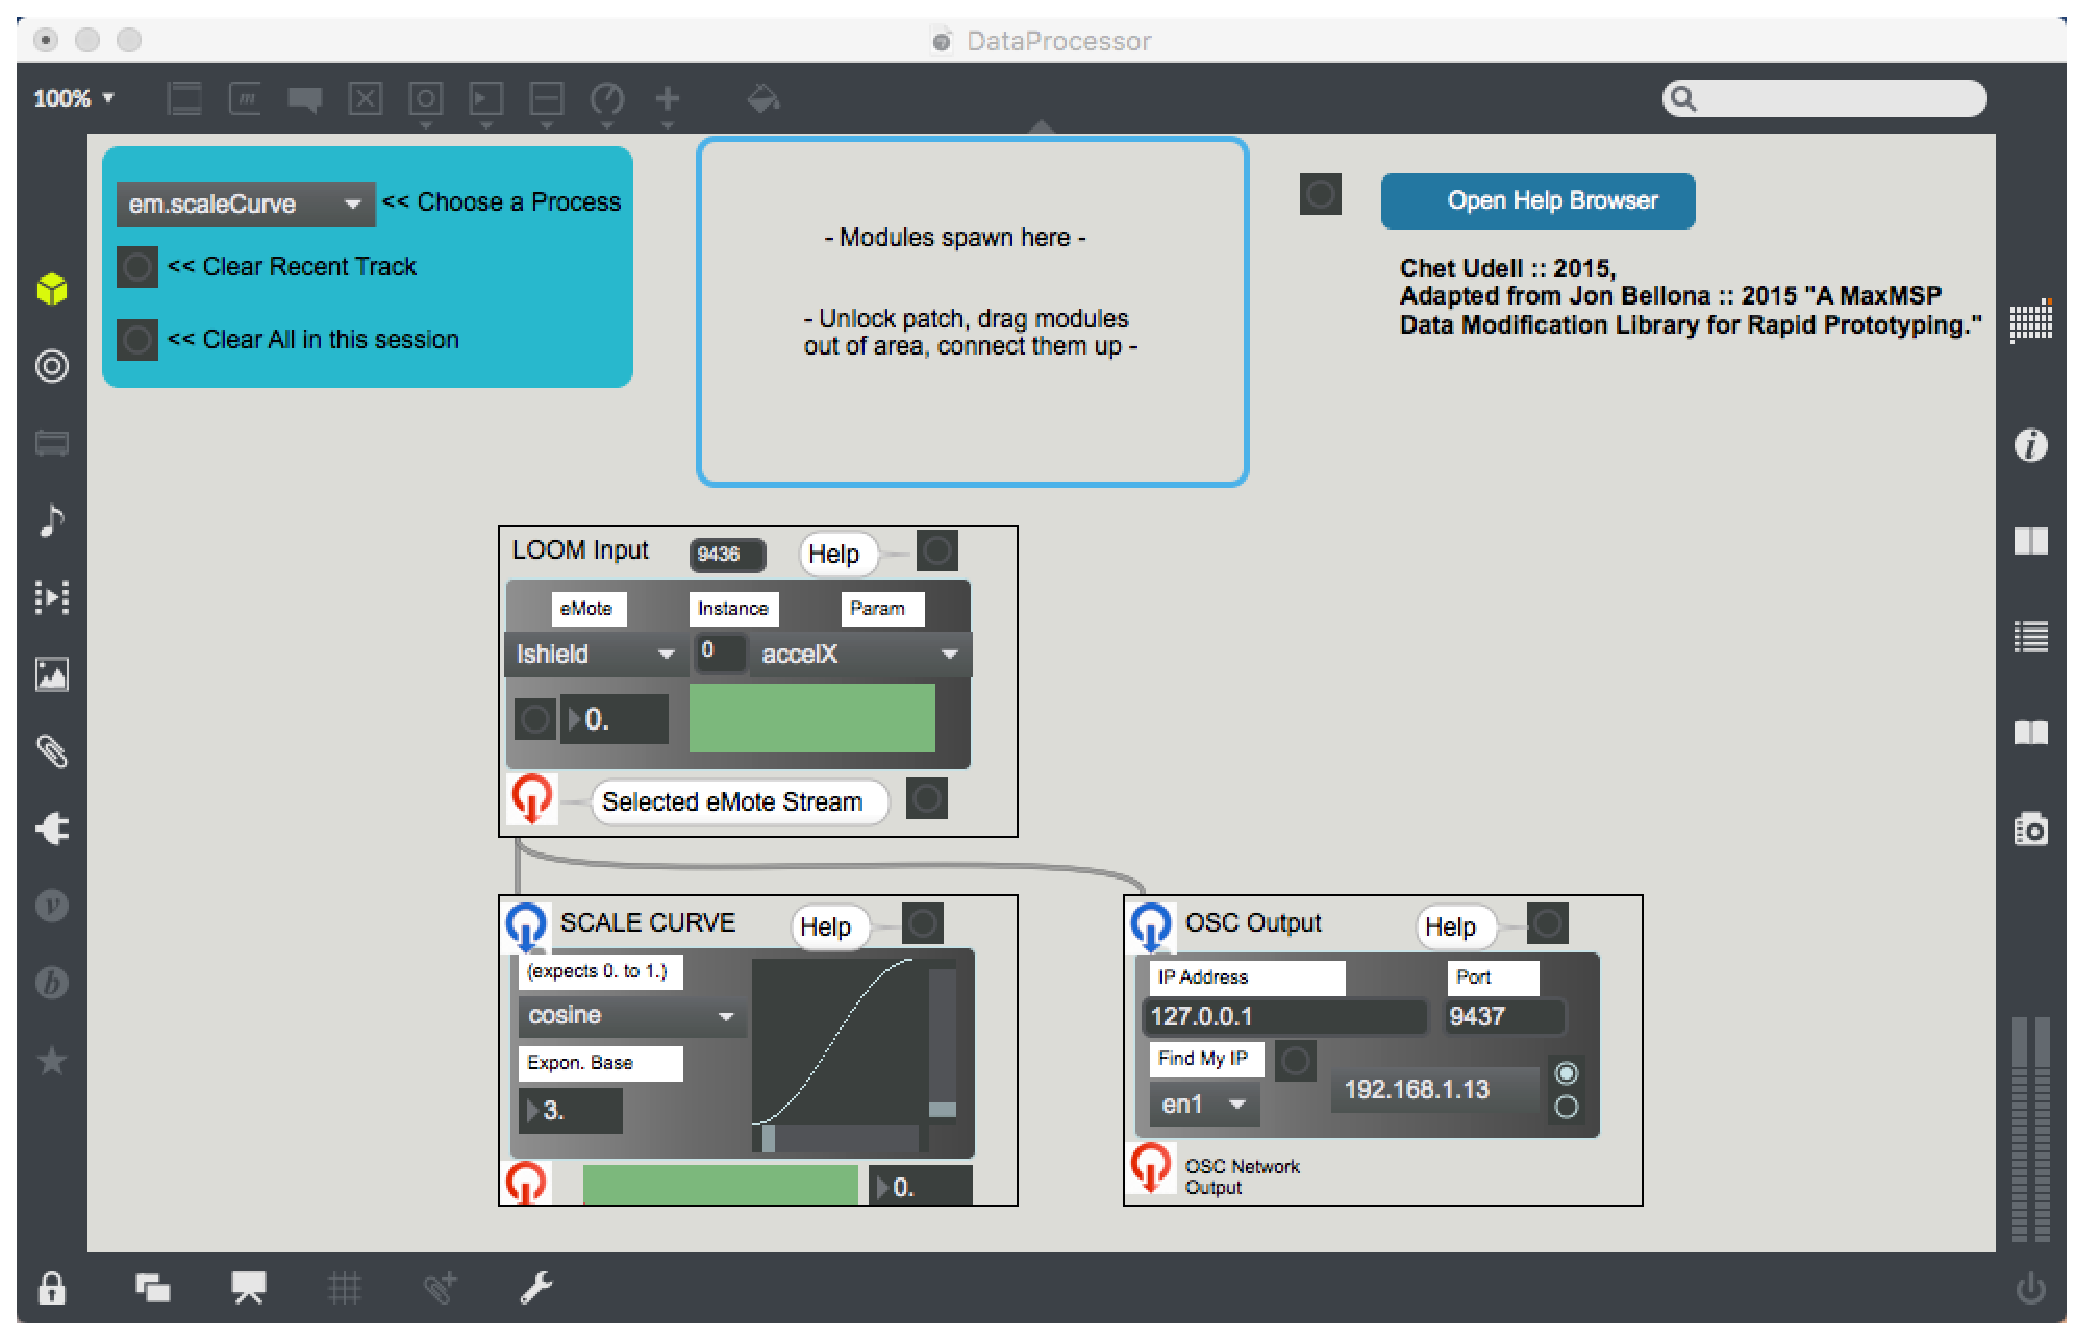
\includegraphics[width=.8\linewidth]{max_example_interface.eps}         
    \end{figure}


\subsubsection*{Trevor}
    \begin{adjustwidth}{2.5em}{0pt}
    \textbf{Summary -} Turned in the requirements document rough draft (will get some questions answered by Chet next week so we can complete it on time in a satisfactory manner), started working on read/write flash functionality with Will, planning to test   next week when we get a chance.
    \end{adjustwidth}
\subsubsection*{William}
    \begin{adjustwidth}{2.5em}{0pt}
    \textbf{Summary -} Met with CS team and Chet on Monday. Met with whole team and Chet on Tuesday. Assigned task to write functionality for reading from and writing to flash memory on M0 boards.

    \textbf{Problems -} Dependencies aren't all on the GitHub.
    \end{adjustwidth}
    \begin{adjustwidth}{5em}{0pt}
    \textbf{Solution -} Went through each sketch and added all dependencies to a dependencies folder which was pushed to the remote repository.
    \end{adjustwidth}

    \begin{listing}[H]    
        \caption{Flash and Debug Code}  
        \label{lst:flash_and_debug}    
    %     % \inputminted[xleftmargin=20pt,fontsize=\small,frame=leftline]{c}{code/_flash_and_debug.tex}


\begin{minted}[xleftmargin=20pt,fontsize=\small,frame=leftline]{c}
//----------------------------------------------------------------------------------------
// DEBUG MODE: Set to 1 to see serial printouts, set to 0 for field use to save memory
//----------------------------------------------------------------------------------------
#ifndef DEBUG
#define DEBUG 1
#endif

//----------------------------------------------------------------------------------------
// MEMORY TYPE: M0 uses flash (MEM_TYPE = 0), 32u4 uses EEPROM (MEM_TYPE = 1)
//----------------------------------------------------------------------------------------
#define MEM_FLASH 0
#define MEM_EEPROM 1

#ifndef MEM_TYPE
#define MEM_TYPE MEM_FLASH
#endif  

...

#if MEM_TYPE == MEM_FLASH
#include <FlashStorage.h>
#endif 

//Structure to store device configuration information
struct config_t {
    byte checksum;               //value is changed when flash memory is written to.
    IPAddress ip;                //Device's IP Address
    char* ssid;                //Created AP's name
    char* pass;                //AP Password (10 or 26 characters long)
    int   keyIndex;            //Key Index Number (needed only for WEP)
    char* ip_broadcast;        //IP to Broadcast data
    unsigned int localPort;      //Local port to listen on
    byte  mac[6];                 //Device's MAC Address
    #ifdef is_i2c
        int   ax_offset, ay_offset, az_offset, gx_offset, gy_offset, gz_offset; //mpu6050 config
    #endif
};
struct config_t configuration;
const byte memValidationValue = 99; // Value to test to see if memory has been written before

#if MEM_TYPE == MEM_FLASH
    FlashStorage(flash_config,config_t);    //Setup the flash storage for the structure
#endif
\end{minted}
\end{listing}



\subsection{Week Six}
\subsubsection*{Luke}
    \begin{adjustwidth}{2.5em}{0pt}
    \textbf{Summary -} The focus this week was on finalizing the client requirements document, as well as some work on firmware (as there is not yet much to do for software - which is my primary role within the project). I will see what I can do regarding the universal thermocouple with Trevor. Juneki asked about the user interface we mentioned in the problem statement so I see him a picture of a sample arrangement of data processors in Max    
    \end{adjustwidth}
\subsubsection*{Trevor}
    \begin{adjustwidth}{2.5em}{0pt}
    \textbf{Summary -} Turned the requirements document in (after implementing the changes and suggestions Chet had to offer). Met with Kenny and went over the source code for the thermocouple shield, will work on adding flash stuff to it once I have Will's code  to base it off.
    \end{adjustwidth}
\subsubsection*{William}
    \begin{adjustwidth}{2.5em}{0pt}
    \textbf{Summary -} Meeting on Monday went well, tasks for the week were given. Meeting on Tuesday was canceled because Chet was busy. Will be meeting with Trevor over the weekend to test the flash memory code. Worked on the requirements document.
    \end{adjustwidth}



\subsection{Week Seven}
\subsubsection*{Luke}
    \begin{adjustwidth}{2.5em}{0pt}
    \textbf{Summary -} There were not many software related items to work on this week, so I continued to help with the firmware side of the project. I also made a short "manual" of how to set up Max (for new users), including those that need legacy 32-bit Java support. I met up with Kenny Noble (from the ECE team of Project LOOM) so that he could demo and show me how he implemented a few different shields. These were the WiFi shield, the thermocouple, and the Loom Ishield with a gyro sensor attached. While the thermocouple functions currently, there was still a little bit of work that Kenny planned to do on it. The older WiFi demo was just a simpler version of the Loom WiFi Ishield that Chet asked me to prepare a demo for. For this, I set up a basic drum kit like demo based on the gyroscopic positioning of the shield. We also started looking into what the technology reviews entail.
    \end{adjustwidth}


    \begin{figure}[H]
        \centering
        \caption{MPU6050 Gyro Drum Demo}
        \label{fig:drum_demo}
        \subfloat[Ishield]{{\includegraphics[width=5cm]{ishield.eps} }}
        \qquad
        \subfloat[Max Visualizers]{{\includegraphics[width=9cm]{drum_demo.eps} }}
    \end{figure}


\subsubsection*{Trevor}
    \begin{adjustwidth}{2.5em}{0pt}
    \textbf{Summary -} Met with Chris Harper, Tom DeBell, Alex Grejux on Thursday to go over the ideal data transfer formats for different networking options (WiFi, LoRa, nRF etc.). Decided that on a low level most of the parsing will be done on a central hub; ideally OSC messages are only sent to/from a hub and a PC, and everything else is sent in a simple byte stream struct containing just enough information to identify the target and the command. Will design further later. Need to start working on OSC parsing driver.
    
    \textbf{Problems -} Need to figure out a good way to make sure low-power devices are able to report their status when they send packets of data.
    \end{adjustwidth}
    \begin{adjustwidth}{5em}{0pt}
    \textbf{Solution -} Possibly have the hub send out a heartbeat that the device responds to when it wakes up? Will discuss this with Chet.
    \end{adjustwidth}
\subsubsection*{William}
    \begin{adjustwidth}{2.5em}{0pt}
    \textbf{Summary -} Met with Chet and CS Team on Monday. Met with Chet and whole team on Tuesday. Continued to work on flash memory. Continued to add to DEBUG functionality. Tested all code on both 32u4 and M0. 
    
    \textbf{Problems -} All the sketches will work on either 32u4 or M0, but for some of the sketches it requires tweaking of the code rather than simply changing the value of a preprocessor definition, or some similar easy configuration change. Testing flash memory is difficult because I do not have an M0 to run the sketch on.
    \end{adjustwidth}
    \begin{adjustwidth}{5em}{0pt}
    \textbf{Solution -} Wrote compilation notes for each of the sketches that require significant code changes to compile on both devices. Checked out an M0 for the week from Chet.
    \end{adjustwidth}



\subsection{Week Eight}
\subsubsection*{Luke}
    \begin{adjustwidth}{2.5em}{0pt}
    \textbf{Summary -} This week we focused on the technology reviews for the class, with peer reviewing for feedback. In terms of project progress, I worked some on getting some progress on sending computer input to the Feather M0 WiFi board - essentially the inverse of the previous demo (sending board gyro to computer). I will finish this Monday before the weekly meeting.
    
    \textbf{Problems -} I was unsure about how to receive data on Feather M0.
    \end{adjustwidth}
    \begin{adjustwidth}{5em}{0pt}
    \textbf{Solution -} Thomas directed me to some code that should be helpful. I also went 
    through the Adafruit Wifi examples/tutorial and was able to better understand what I needed to do.   
    \end{adjustwidth}
\subsubsection*{Trevor}
    \begin{adjustwidth}{2.5em}{0pt}
    \textbf{Summary -} Got technology review peer reviewed by my classmate John Magenheimer. Chet was busy for Monday's meeting and I was unable to attend the Tuesday meeting, but I still managed to work on a few template files for generalizing the source code for the different WiFi shields.
    \end{adjustwidth}
\subsubsection*{William}
    \begin{adjustwidth}{2.5em}{0pt}
    \textbf{Summary -} Met on Monday with Thomas (rather than Chet, who was busy) to go over the progress each of the CS team members has made, and to prepare for the meeting on Tuesday. Met on Tuesday to discuss the overall progress of the project. Met on Thursday with Chris Harper to discuss LoRa, nRF, and merging my branch containing memory and debug code with the master.
    \end{adjustwidth}



\subsection{Week Nine}
\subsubsection*{Luke}
    \begin{adjustwidth}{2.5em}{0pt}
    \textbf{Summary -} This week I focused on getting Max to send data to a Feather M0 Wifi board. To demonstrated this, I used a NeoPixel (tri-color LED) and used sliders in Max to control the RGB values that the NeoPixel displayed. Chet also showed me how to make new data processor plugins in the format that he used to make his. We were able to send commands to the board via simple UDP strings and OSC packets. 
    \end{adjustwidth} 

    \begin{figure}[H]
        \centering
        \caption{Neopixel Demo}
        \label{fig:neopixel_demo}
        \subfloat[Max Neopixel Processor]{{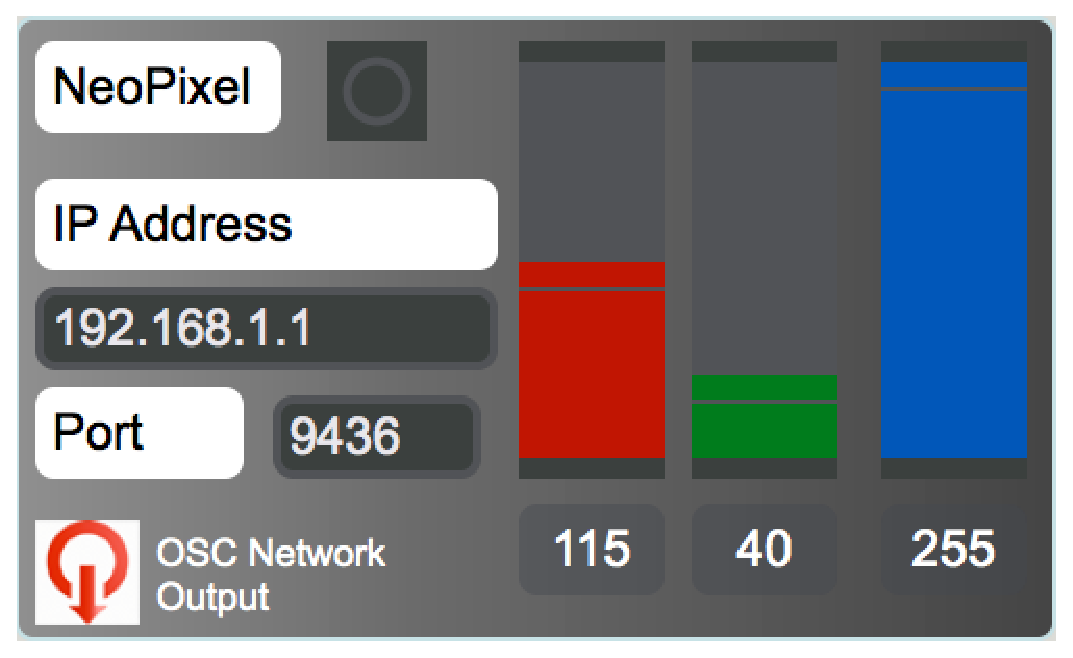
\includegraphics[width=6cm]{neopixel_pres.eps}}}
        \qquad
        \subfloat[Ishield with NeoPixel]{{\includegraphics[width=6cm]{ishield_neopixel.eps}}}
    \end{figure}

    \begin{figure}[H]
        \centering
        \caption{Edit Neopixel Max Module}
        \label{fig:neopixel_edit}
        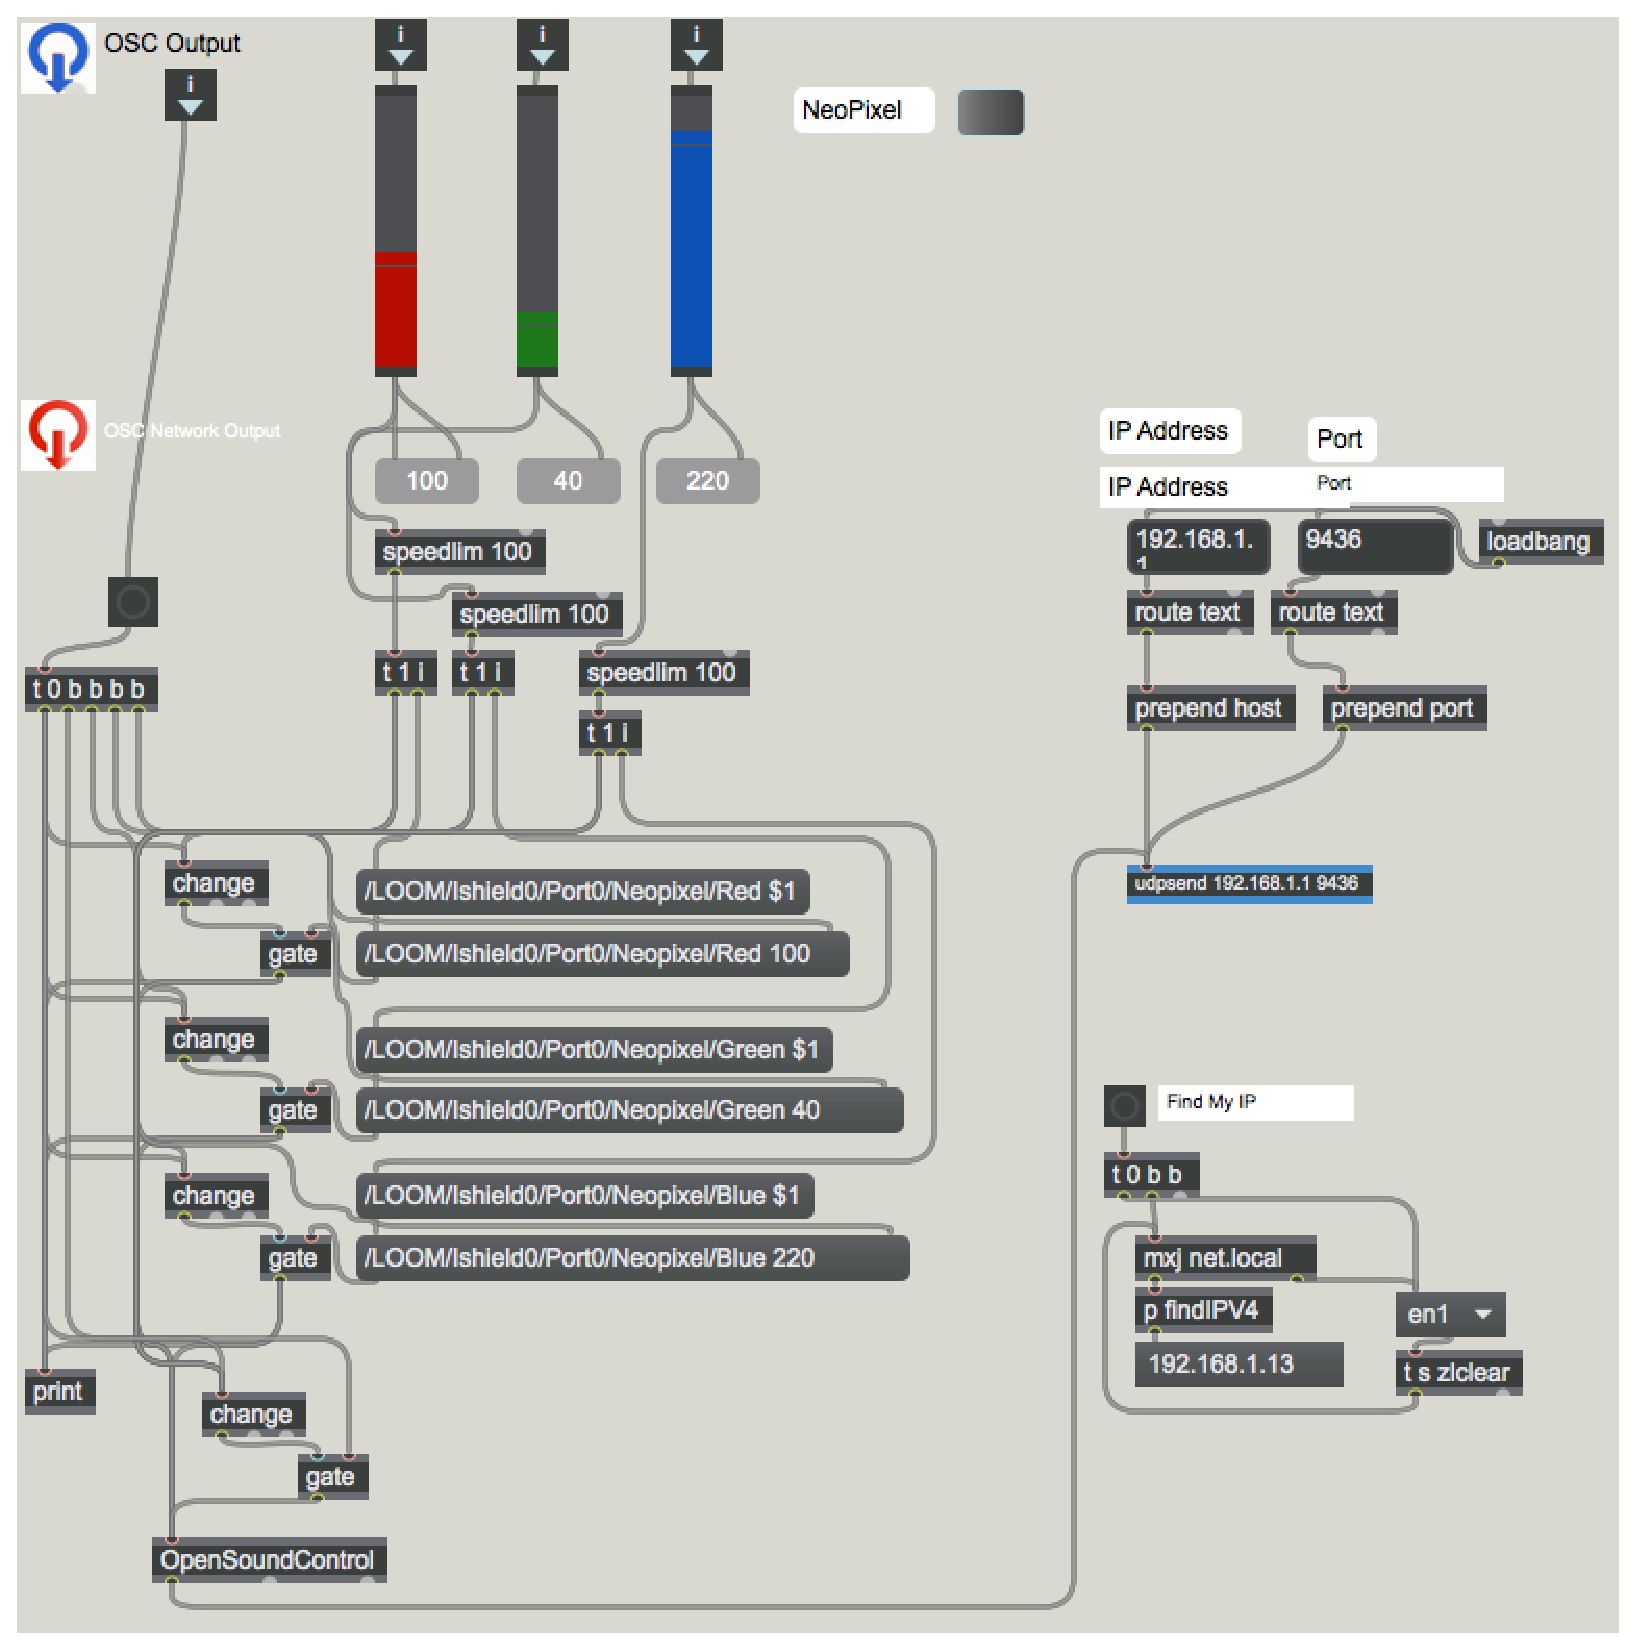
\includegraphics[width=10cm]{neopixel_edit.eps}
    \end{figure}


\subsubsection*{Trevor}
    \begin{adjustwidth}{2.5em}{0pt}
    \textbf{Summary -} Met with Chet, Will, and Luke on Monday, met with overall team on Tuesday. Turned in the tech review. Worked with Will a little bit on the flash code. I met with Luke and we got the NeoPixel to receive and interpret OSC bundles.
    
    \textbf{Problems -} I was out of town most of the week for Thanksgiving/my cousin's wedding so I did not get a lot done.
    \end{adjustwidth}
    \begin{adjustwidth}{5em}{0pt}
    \textbf{Solution -} Returned from Thanksgiving.
    \end{adjustwidth}
\subsubsection*{William}
    \begin{adjustwidth}{2.5em}{0pt}
    \textbf{Summary -} Met with Chet and CS team on Monday. Met with Project LOOM Team on Tuesday. Continued to work on Flash Memory. Successfully pushed my changes to the remote master. Assigned task to restructure flash memory code to calibrate the MPU6050 when no values are stored in flash memory. The MPU6050 must also be able to receive commands in the form of OSC bundles.
    
    \textbf{Problems -} Had difficulty testing the OSC bundle receiving because I did not have the MaxMSP program necessary to send the bundles.
    \end{adjustwidth}
    \begin{adjustwidth}{5em}{0pt}
    \textbf{Solution -} Got the program from Luke and Trevor. Will start testing next week.
    \end{adjustwidth}



\subsection{Week Ten}
\subsubsection*{Luke}
    \begin{adjustwidth}{2.5em}{0pt}
    \textbf{Summary -} This week, I focused on improving and expanding upon the NeoPixel demo, and altering the programs/modules to work with other actuators, namely, a servo. Both the NeoPixel and the servo now receive proper OSC bundles instead of just separate messages. I will continue to work on getting the NeoPixel to change color based on orientation over the weekend.    
    \end{adjustwidth}
\subsubsection*{Trevor}
    \begin{adjustwidth}{2.5em}{0pt}
    \textbf{Summary -} This week, we completed and turned in the design document. Also worked on a generic template for devices that will use the OSC message routing system to dispatch functions based on the message address. I met with Dongjun Lee, from the ECE capstone team, and worked on getting the Servo shields to receive OSC bundles with commands for individually addressable servos, and successfully got that working with a prototyped MaxMSP data processor plugin. Also met with Will and we got the OSC calibration command setup for the MPU6050 shield.
    
    \textbf{Problems -} May in fact want to take an M0 home over break.
    \end{adjustwidth}
    \begin{adjustwidth}{5em}{0pt}
    \textbf{Solution -} Will check out an M0 from the lab so I can test all the things.
    \end{adjustwidth}


    \begin{figure}[H]
        \centering
        \caption{Servo Demo}
        \label{fig:servo_demo}
        \subfloat[Max Servo Processor]{{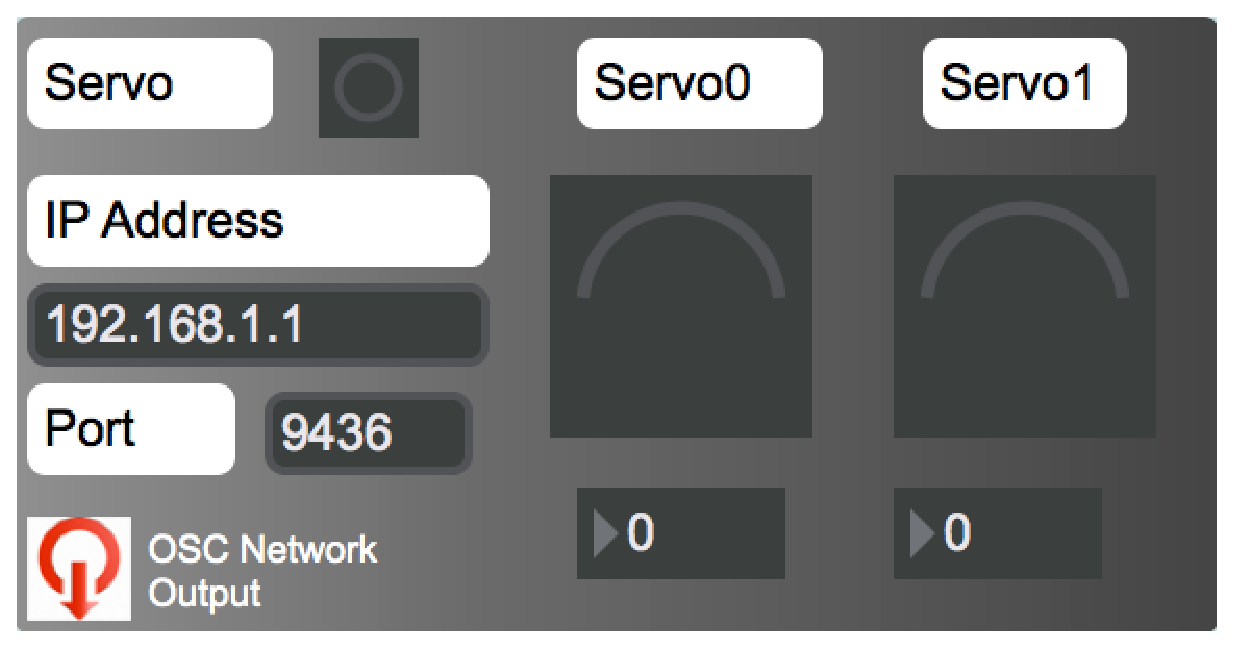
\includegraphics[width=6cm]{servo_pres.eps}}}
        \qquad
        \subfloat[Ishield with NeoPixel]{{\includegraphics[width=6cm]{servo.eps}}}
    \end{figure}


    \begin{listing}[H]    
        \caption{OSC Bundle Reception} 
        \label{lst:osc_bundle_reception} 
        \begin{minted}[xleftmargin=20pt,fontsize=\small,frame=leftline]{c}
void loop() {
    OSCBundle bndl;

    int packetSize = Udp.parsePacket();
    if (packetSize > 0){
    Serial.println("=========================================");
    Serial.print("received packet of size: ");
    Serial.println(packetSize);
    while (packetSize--){
        bndl.fill(Udp.read());
    }
    if (!bndl.hasError()){
        bndl.route("/LOOM/ServoShield0",handleServo);
    }
    else {
        error = bndl.getError();
        Serial.print("error: ");
        Serial.println(error);
        }
    } 
}
        \end{minted}
        % \inputminted[xleftmargin=20pt,fontsize=\small,frame=leftline]{c}{code/_osc_bundle_reception.tex}
    \end{listing}


    \begin{listing}[H]    
        \caption{Servo OSC Interpretation Code} 
        \label{lst:servo_interpret_osc}   
        \begin{minted}[xleftmargin=20pt,fontsize=\small,frame=leftline]{c}
void handleServo(OSCMessage &msg, int addrOffset){
    int degree;
    degree = msg.getInt(0);
    if (msg.fullMatch("/Servo0/Set",addrOffset))
        set_servo_degree(degree,0);
    #if num_servos > 1
        else if (msg.fullMatch("/Servo1/Set",addrOffset))
            set_servo_degree(degree,1);
    #endif
    #if num_servos > 2
        else if (msg.fullMatch("/Servo2/Set",addrOffset))
            set_servo_degree(degree,2);
    #endif
      // ADD checks for matching on Servo2, Servo3, etc.
}
        \end{minted} 
        % \inputminted[xleftmargin=20pt,fontsize=\small,frame=leftline]{c}{code/_servo_interpret_osc.tex}
    \end{listing}

\subsubsection*{William}
    \begin{adjustwidth}{2.5em}{0pt}
    \textbf{Summary -} Met with CS Team and Chet on Monday. Met with whole team on Tuesday. Tested out OSC bundle reception with Trevor. Code for calibration after receiving a specific command in an OSC bundle works.Once bundle parsing is more structured, will merge with master then push when ready.
    
    \textbf{Problems -} Need to talk to Chet about maybe bringing home an M0 during Winter break to continue working. 
    \end{adjustwidth}



\section{Retrospective}

\begin{center}
\begin{longtable}{|p{0.3\linewidth}|p{0.3\linewidth}|p{0.3\linewidth}|} 
% \noindent
% \begin{tabularx}{|p{0.3\linewidth}|p{0.3\linewidth}|p{0.3\linewidth}| } 
% \begin{tabularx}{0.9\linewidth}{|p{0.3\linewidth}|p{0.3\linewidth}|p{0.3\linewidth}| } 

 \hline
 \textbf{Positives} & \textbf{Deltas} & \textbf{Actions} \\ 
 \hline
 The collective group of Project LOOM is well organized and communication is good, keeping progress steady. & A more structured method or architecture for parsing OSC Bundles on the receivers should be developed. & The Firmware/Embedded team will communicate with Chet before and possibly during Winter break to continue the development of a modular bundle parsing system that can be included in any sketch.  \\ 
 \hline
 Luke and Trevor developed a working MaxMSP module that allows for easy testing of Arduino sketch OSC bundle parsing functionality. & Add more modules and extend the functionality of the existing modules to work with different network setups; currently it works over a WiFi connection but we eventually want ethernet, LoRa, nRF, and as a stretch goal Bluetooth & First, develop generic templates and headers for each of these different networks, then integrate them into the currently functioning shields. \\ 
 \hline
 Got the required firmware for a proof of concept, and all three required modules done for Chet’s Honors class in Winter term. & We will need to develop and implement the architecture and functionality for usage of gateways in LOOM networks & We will continue to discuss with Chet and Chris Harper (the people on the gateway team) about what their plans for the architecture are. Once a plan for architecture has been drawn up, we will work on changing the structure of the existing sketches to work with the new gateway architecture. \\ 
 \hline
 The project is well setup to transition to the use of individual gateways rather than having modules function as access points. &  &  \\ 
 \hline
\end{longtable}
\end{center}

% \nocite{*}
% \bibliographystyle{IEEEtran}
% \bibliography{bib}

\end{document}